Agisoft Metashape can approximate the camera parameters automatically, but to get an accurate reconstruction of the object we include the intrinsic camera parameters. The parameters can be given for each image individually or we can create groups of images and impose the same parameters for all the images in the group. The intrinsic parameters are calculated form the CHAVORE[ref] data that is provided for all the images in the $.xml$ files. The parameters are form[ref] which is scripted in python[1]. The input parameters are $f, k1, k2, k3, cx, cy$, as seen in \ref{fig:cameraCalibrationMetashape} which is the focal length, distortion coefficent and the principal point of the images.
\begin{lstlisting}[language=xml, caption=xml file, label=xmlFile]
<?xml version='1.0' encoding='UTF-8'?>
<calibration>
  <projection>frame</projection>
  <width>1648</width>
  <height>1200</height>
  <f>14771.071671547474</f>
  <cx>-0.3312798406959963</cx>
  <cy>1.0928099206940067</cy>
  <k1>0.000193151</k1>
  <k2>1.8354094491035e-09</k2>
  <k3>8.081357601557738e-19</k3>
</calibration>
\end{lstlisting}
\begin{figure}[H]
	\centering
	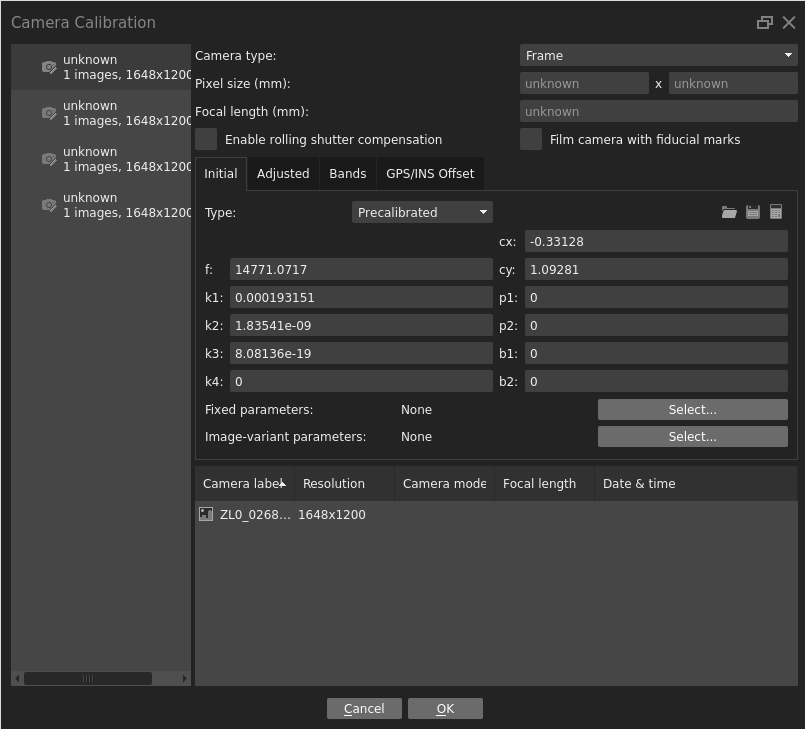
\includegraphics[scale=0.3]{img/cameraCalibration.png}
	\caption{Callibration Parameters}
	\label{fig:cameraCalibrationMetashape}
\end{figure}
These parameters are stored in a $.xml$ file by using a script[ref] that converts the data to xmls, as agisoft allows us to upload the parameters through a file \ref{xmlFile} instead of manually entering all the values. The option to upload the file can be found on \ref{fig:cameraCalibrationMetashape} for each selected image.
\begin{figure}[H]
	\centering
	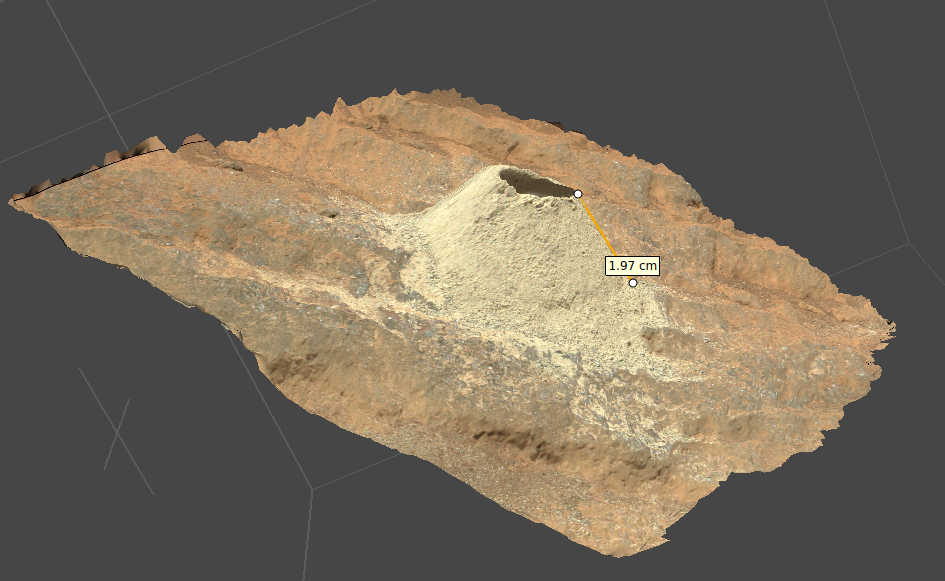
\includegraphics[scale=0.3]{img/drill.png}
	\caption{Sol-268 with Parameters}
	\label{fig:drillHole}
\end{figure}
This makes the alignment process more accurate and the model that we get will be scaled to the actual size of the object as seen in \ref{fig:drillHole}. As in Uncalibrated reconstruction without the parameters we do not get an exact dimesion of the reconstructed object. When dealing with multiple images the process of selecting the xmls for them can be automated with a python script. All processes in agisoft can be maniputed using the python metashape package in a script, this reduces the process of uploading the data for each image when dealing with reconstruction that involves multiple images.

